\documentclass[parskip=full]{scrartcl}
\usepackage[table,xcdraw]{xcolor}

\pagenumbering{gobble}      % turn off page numbering for titlepage and index
\usepackage[utf8]{inputenc} % use utf8 file encoding for TeX sources
\usepackage[T1]{fontenc}    % avoid garbled Unicode text in pdf
\usepackage[german]{babel}  % german hyphenation, quotes, etc
\usepackage{hyperref}       % detailed hyperlink/pdf configuration
\hypersetup{                % ‘texdoc hyperref‘ for options
	pdftitle={Algorithmen für Planare Graphen SS2019},
	bookmarks=true
}
\usepackage{graphicx}       % provides commands for including figures
\usepackage{csquotes}       % provides \enquote{} macro for "quotes"
\usepackage[nonumberlist]{glossaries}     % provides glossary commands
\usepackage{enumitem}
\usepackage{wrapfig}
\usepackage{amssymb}        % Für Textumfluss
\usepackage{pifont}
\usepackage{tikz}
\usetikzlibrary{graphs,graphs.standard}

\makeglossaries

\title{Algorithmen für Planare Graphen}
\subtitle{Inoffizieller Mitschrieb der Vorlesung im Sommersemester 2019}
\author{Andreas Mai}
\date{} % Remove Date
%\institute{Karlsruher Institut für Technologie}

\begin{document}

\maketitle
\begin{center}
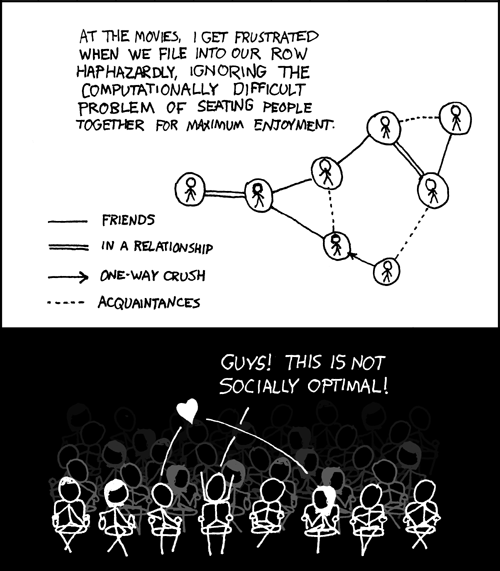
\includegraphics[scale=0.7]{movie_seating}\\
\url{https://xkcd.com/173}
\end{center}

\clearpage
\tableofcontents
\pagenumbering{arabic}
\setcounter{page}{1}

\textbf{Disclaimer: } \\
Dies ist ein inoffizieller Mitschrieb.\\
Ich übernehme keine Haftung auf die Korrektheit der Inhalte.

\clearpage

\section{Organisatorisches}
\begin{itemize}
  \item \textbf{Das offizielle Skript auf der Homepage ist teilweise veraltet!\\ siehe Prüfungsprotokolle}
  \item Vorlesungshomepage\\
  \url{https://i11www.iti.kit.edu/teaching/sommer2019/planar_graphs/index}
\end{itemize}
\section{Einführung}



\iffalse % Added later
\section{Kuratowski}
  \begin{figure}
    \centering
    \begin{tikzpicture}
      \graph[empty nodes, nodes={circle,draw}]{ subgraph K_n [n=5,clockwise,radius=2cm] };
    \end{tikzpicture}
    \caption{$K_5$ Graph}
  \end{figure}
\fi

\end{document}